\documentclass[UTF8]{ctexart}
\usepackage[top=2.54cm, bottom=2.54cm, left=3.18cm,right=3.18cm]{geometry}  %与a4纸大小相同
\usepackage{indentfirst}   %首行缩进
\usepackage{graphicx}
\usepackage{amsmath}
\usepackage{listings}  %插入代码
\usepackage{float}    %使插图的位置不跑到开头而紧跟插入的文字后,插入图片时后加H
\fontsize{15.75pt}{24pt}\title{\textbf{对旅行商问题多重解答的探讨}} 
\date{}
\pagestyle{plain}      %无页眉,只有页码的中间页脚

\begin{document}

	\maketitle
	\fontsize{14pt}{24pt}\begin{center}
		\textbf{摘要:}
	\end{center}
	
	\fontsize{12pt}{24pt}
	
	本文主要对典型的旅行商(Traveling salesman problem)问题进行了分析,并尝试使用蚁群算法、模拟退火算法以及遗传算法多种算法用matlab对其实现了解答。
	
	由于TSP是一个典型的组合优化问题,而lingo软件的长处就在于求解优化类问题,并且具有输入模型简练直观、运行速度快、引入了集合的概念等特点,因此我们尝试使用lingo软件描述出了tsp问题,并对其进行了求解。
	
	为了将4种方法进行比对分析,我们对每种算法采用了相同的城市坐标数据。经过分析,我们得到以下结论:
	
	1.lingo是4种方法里面最容易描述TSP问题的。它仅需输入数据、约束条件以及目标函数,即可自动选择合适的求解器。对于TSP问题,它采用了B—and—B求解器,即分枝定界算法。lingo求得的目标函数值最为精确。而lingo相比matlab的缺陷在于,它的运行时间较长,显著多于matlab的算法,在运行效率上有着较大的劣势。而且它不能实现最短路径的可视化,在描述运算结果方面不如matlab直观。
	
	2.lingo的求解稳定性是4者当中最优的。多次重复运行同样的代码,所得的计算结果以及运行所用时间均无明显变化。
	
	3.不论采取何种算法,matlab相比lingo,都有着可以实现城市位置以及具体线路的可视化的优势,这使得计算结果更加直观。
	
	4.模拟退火算法是matlab3种算法计算效率最高的,计算结果也略优于其他几个算法,这证明了模拟退火算法的可靠性与有效性。
	
	
	5.蚁群算法的运行速度仅次于模拟退火算法,但是它的解的质量不如模拟退火算法和lingo的。
	
	6.遗传算法的运行时间是3种matlab算法中最长的,且解的质量是4种方法里面最低的。这说明代码尚有较大的优化空间。
	
	7.综上可知,我们讨论的4种方法中,对TSP问题适应性最好的是模拟退火算法,其次是lingo。最需要改进的是遗传算法。

	\vspace{60pt} 
	
	
	\textbf{关键词:旅行商问题{ }{ }{ }模拟退火算法{ }{ }{ }蚁群算法{ }{ }{ }遗传算法{ }{ }{ }lingo编程}
	\newpage
	\fontsize{14pt}{24pt}\textbf{\begin{center}
			一、 问题重述
	\end{center} }
	
	\fontsize{12pt}{24pt}
	题目要求:已知一些点的位置以及它们之间相互的距离,求遍历所有点、且不重复经过任何一个点的距离最短的路线。
	
	
	这本质上是一个旅行商问题(Traveling salesman problem)。TSP问题如下:一名商品推销员要去若干个城市推销商品,该推销员从一个城市出发,需要经过所有城市后,回到出发地。问应当如何选择行进路线,以使总的行程最短。
	
	可见,两者的数学模型是一模一样的。我们只需对其中任意一个进行求解,另外一个也会得到解答。故下面我们直接对TSP问题进行分析与解答。
	
	\vspace{150pt}
	
	
	
	\fontsize{14pt}{24pt}\textbf{\begin{center}
			二.对问题的初步分析
	\end{center} }
	
	\fontsize{12pt}{24pt}
	旅行商问题是组合优化中的一个非线性规划(NP)困难问题,该问题的求解与计算均有不低的难度。
	
	若题中的城市数量较少,我们可以采用枚举的方式,穷举出所有可能的路径并一一计算相应的距离,之后即可进行比对选取总距离最短的路径。
	
	然而,随着城市数目的增加,会产生计算量爆炸的情形,导致计算机难以对其进行求解。因此我们需要寻找更加高效、有针对性的解题方式。
	
	查询资料可知:常用的算法主要为近似算法或启发式算法,主要有遗传算法、模拟退火法、蚁群算法、禁忌搜索算法、贪婪算法和神经网络等。本文我们主要尝试使用matlab以蚁群算法、模拟退火算法、遗传算法以及lingo对TSP问题进行求解。最后运行的结果表明,这四种方式确实均是可以实现的。四种求解方法的优劣势均在下文中得到了具体的探讨。
	
	
	
	

	
	

	\newpage
	
	
	\fontsize{14pt}{24pt}\textbf{\begin{center}
			三、MATLAB使用蚁群算法解TSP问题
	\end{center} } 
	
	\fontsize{14pt}{24pt}\textbf{\begin{flushleft}
			3.1蚁群算法的原理
	\end{flushleft}}
	\fontsize{12pt}{24pt}蚁群算法是一种基于信息正反馈原理的算法。它采用了仿生的形式,通过对蚂蚁群体选择觅食路径的方法的学习,实现了与现实问题的结合,并在许多问题的求解上取得了显著的效果。
	
	自然界中的蚂蚁视觉十分不灵敏,但是它却总是能在缺乏提示的条件下自动选择到从食物源到食物储存地的最短路径。这是因为每一只蚂蚁在寻找食物的路途中,总是会在路上释放信息素,使得相邻的一定范围内的其他蚂蚁可以较为容易地察觉到这条路径的存在。当经过某一条路径的蚂蚁数量增多时,该路径上的信息素浓度会相应地上升,从而吸引更多蚂蚁来走这条路,进而促使该路径信息素浓度不断上升,形成一个正反馈的机制。
	
	在现实中,信息素浓度在没有其他蚂蚁持续供应的情况下,会由于各自外界原因(如雨水的冲洗)而减弱。在将蚁群的行为进行仿生的过程中,也应该考虑到这个因素。
	
	
	
	\fontsize{14pt}{24pt}\textbf{\begin{flushleft}
			3.2蚁群算法TSP模型的建立
	\end{flushleft}}
	\fontsize{12pt}{24pt}假设蚂蚁会且仅会在每个城市之间的连线的线路上经过,蚂蚁总数量为m,城市数量为n,城市i与城市j之间的距离为$d_{ij}$,t时刻城市i与城市j连接路径上信息素浓度为$\tau_{ij}(t)$.初始时刻,各蚂蚁均匀分布在不同的城市,且各城市路径上的信息素浓度相同,均为$\tau_{ij}0=\tau_{0}$。之后蚂蚁会按照一定的概率选择线路,设$p_{ij}^{k}$为t时刻蚂蚁k从城市i移动到城市j的概率。而蚂蚁选择线路主要受到以下2个方面的影响,一是访问某城市的期望值,二是线路上的信息素浓度。我们令:
	$$ p_{ij}^{k}=\left\{
	\begin{aligned}
	 & \frac{[ \tau_{ij}(t)]^\alpha*[\eta_{ij}(t)]^\beta}{\sum_{s \in allow_{k}}[\tau_{is}(t)]^\alpha*[\eta_{is}(t)]^\beta},j \in allow_{k}\\
	 & 0,j \notin allow_{k} 
	\end{aligned}
	\right.
	$$
	其中,$\eta_{ij}(t)$为启发函数,表示蚂蚁从城市i转移到城市j的期望程度;$ allow_{k}$为蚂蚁k待访问的城市集合。起初,$ allow_{k}$中有n-1个元素,随着时间推移,它会逐渐减小,直至减为0;$\alpha$为信息素因子,它的值的大小与信息素强度影响正相关;$\beta$为启发函数重要程度因子,它的值的大小与信息素强度影响正相关。
	
	由3.1的原理知,信息素浓度会一定程度上自发降低。令$\rho(0<\rho<1)$表示信息素的挥发程度。则当蚂蚁将所有的城市走完,信息素浓度为
	$$\left\{
	\begin{aligned}
	& \tau_{ij}(t+1)=(1-\rho)*\tau_{ij}(t)+\Delta\tau_{ij}\\
	& \Delta\tau_{ij}=\sum_{k=q}^{m}\Delta\tau_{ij}^k
	\end{aligned}
	\right.$$
	其中,$\Delta\tau_{ij}^k$为第k只蚂蚁在城市i与j连接路径上面释放信息素而使得其增加的浓度大小;$\Delta\tau_{ij}$为所有蚂蚁在城市i与j连接路径上面释放信息素而使得其增加的浓度大小
	
	而$$\Delta\tau_{ij}^k=
	\left\{
	\begin{aligned}
	& \frac{Q}{\L_{k}}\\
	& 0
	\end{aligned}
	\right.
	$$	
	Q为信息素常数,表示蚂蚁经过一次所释放的信息素总量;$\L_{k}$为第k只蚂蚁经过路径的总长度。
	\fontsize{14pt}{24pt}\textbf{\begin{flushleft}
			3.3matlab实现蚁群算法-TSP模型的具体操作
	\end{flushleft}}
	\fontsize{12pt}{24pt}
	matlab对蚁群算法的具体实现方式可以分为以下五步:
	
	1.准备数据:
	
	首先清空环境变量,并开始计时。其次,使用xlsread函数读入所有城市的坐标值并将其保存在citys矩阵中。
	
	
	2.计算城市之间的距离:
	
	使用for函数求出每2个城市之间的距离,并记录在矩阵D中。为了保证启发函数的分母不为0,我们将D的对角线上的所有元素由原先的0修改为足够小的正数:1e-4。
	
	3.初始化参数:
	
	首先,我们将蚂蚁数量、信息素重要程度因子、启发函数重要程度因子与信息素挥发因子等参数赋予一个合适的值。然后,我们将信息素矩阵、路径记录表、最大迭代次数等参数初始化为0或1或其他便于存储的数据。
	
	
	
	4.迭代寻找最佳路径。这是整个算法中的最核心的一部分,是决定整个程序优劣的关键因素。
	
	设置一个while循环,当迭代次数等于最大次数时,则跳出循环,否则,依次进行以下几步。首先,用randperm函数随机产生各个蚂蚁的起点城市,构造m*1的列向量start记录各个蚂蚁的起点位置,用$city_index$表示城市列表。然后,依次按照每只蚂蚁和每个城市进行循环,用tabu矩阵表示禁忌表,即每一次循环时都将前一次经过的城市编号记录上去。而剩下的城市序号则记录在allow矩阵中。可知,随着迭代次数的增加,tabu矩阵中实际表示的城市会越来越多,allow矩阵中实际表示的城市会越来越少,直至循环终止(即每一只蚂蚁都经过了所有城市)。根据3.2提到的函数求解蚂蚁访问下一个城市的概率,再使用轮盘赌法决定每一只蚂蚁的下一个访问城市。
	
	当该2个循环结束后,求得每一次while循环的所有路径长度的平均值。使用Length列向量记录每一只蚂蚁经过的路径之和,并比较while循环前一次所得到的结果,得到当前最短路径的城市序号的顺序、当前最短路径的距离。
	
	为了更进一步地贴合实际并且提高算法质量,我们需要更新信息素浓度。设置两个for循环,依次对每只蚂蚁与对每个城市进行循环,每一次都使用3.2提到的信息素浓度求解函数更新相应节点的信息素浓度。随后将路径记录表清空。
	
	信息素更新完之后,使while迭代次数iter数量增加1,并判断是否达到最大循环次数。若已经达到,则跳出while循环,否则进行下一次循环。
	
	
	
	
	
	
	
	
	5.结果显示:
	
	首先,输出最短距离、最短路径的城市序号、收敛迭代次数以及程序执行时间。随后用plot函数作图,表现出蚁群算法的最优化路径与算法收敛轨迹。
	
	
	
	蚁群算法应用到TSP问题中的代码的思路的流程框图如下:
	\begin{figure}[H]
		\centering
		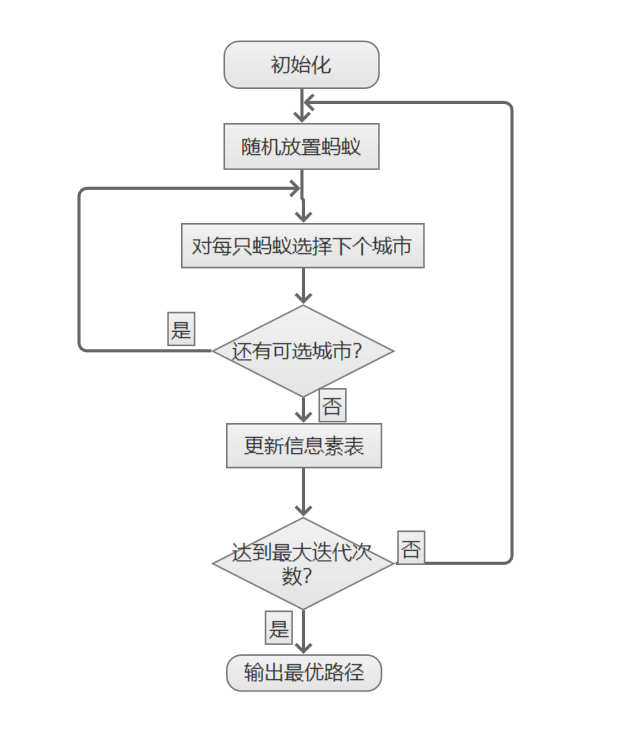
\includegraphics[width=0.7\linewidth]{蚁群算法结构程序框图}
		\caption{蚁群算法结构程序框图}
		\label{fig:}
	\end{figure}
	
	
	
	\fontsize{14pt}{24pt}\textbf{\begin{flushleft}
			3.4对蚁群算法求解结果的展示与分析
	\end{flushleft}}
	\fontsize{12pt}{24pt}
	输出结果如下:
	
	最短距离:7677.6608
	
	最短路径:46 { } 44 { } 34 { } 35 { } 36{ }  39{ }  40{ }  38  { }37  { }  48  { } 24  { }  5  { } 15  { }  6  { }  4 { }  25 { }  12{ }   28  { } 27 { }  26 { }  47 { }  13 { }  14 { }  52 { }  11  { } 51 { }  33 { }  43 { }  10  { }  9 { }   8 { }  41{ }   19 { }  45 { }  32 { }  49 { }   1 { }  22{ }   31{ }   18{ }    3 { }  17{ }   21 { }  42  { }  7 { }   2{ }   30 { }  29 { }  50 { }  20  { } 23 { }  16 { }  46
	
	收敛迭代次数:73
	
	程序执行时间:20.348秒
	
	蚁群算法最优化路径如下:
	\begin{figure}[H]
		\centering
		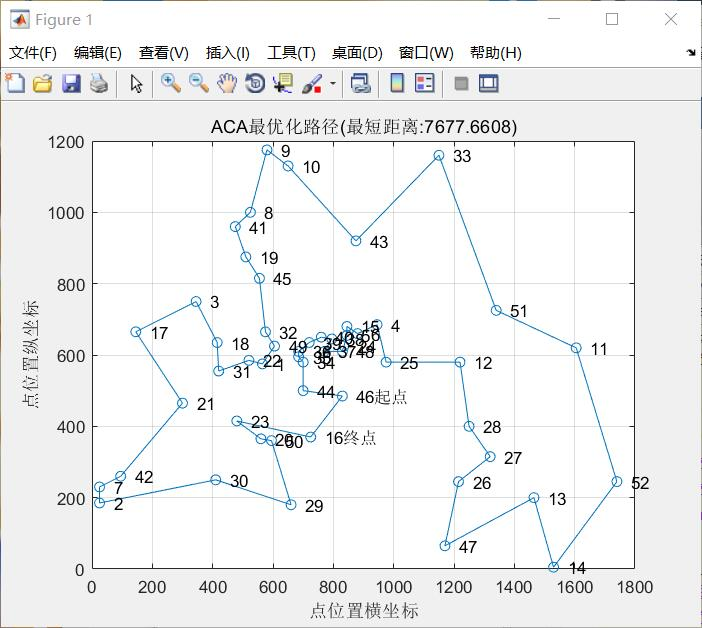
\includegraphics[width=0.7\linewidth]{蚁群算法最优化路径}
		\caption{蚁群算法最优化路径}
		\label{fig:}
	\end{figure}
	蚁群算法收敛轨迹如下:
	\begin{figure}[H]
		\centering
		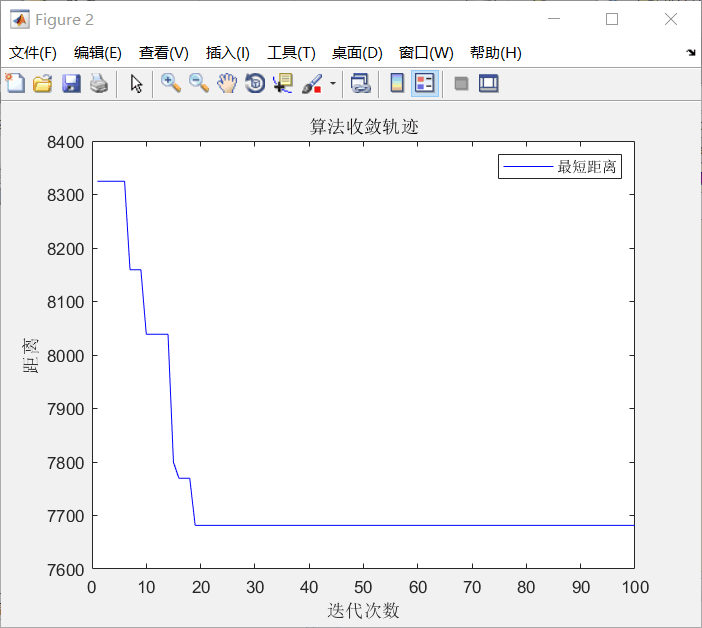
\includegraphics[width=0.7\linewidth]{蚁群算法收敛轨迹}
		\caption{蚁群算法收敛轨迹}
		\label{fig:}
	\end{figure}
	
	结果分析:程序执行时间为20.348秒,在可以接受的时间范围内即完成了如此复杂的计算,证明了蚁群算法的有效性。
	
	反复多次运行同样的代码,运行时间分别为22.256秒,21.183秒,20.091秒,19.827秒,最短路径长度分别为7681.4537,7774.2519,7681.4537,7681.4537。
	
	蚁群算法表现出了一下特点:
	
	1.它并非强求全局最优解,而是会满足于一个质量相对较高的局部最优解。
	
	2.起初算法的收敛速度较快,但是随着迭代次数的增加,收敛速度显著降低,甚至会在测试中出现停滞的情况。
	
	3.蚁群算法对TSP问题有较好的适应性,无论数据规模大小,均能在一定时间内得到较高质量的解。
	
	4.稳定性较差,即便不改变参数,也可能前后运行的结果迥异。为了提高解的质量,不妨采用同样的参数运行5遍以上,选取其中最优解。
	
    5.算法中参数较多,参数的微小调动可能对运行结果的质量、运行时间等产生意外的影响。例如,若蚂蚁数量m值过大,则会导致搜索路径上的信息素量变化趋于平均,正反馈作用被削弱,导致收敛速度减慢。若m过小,则在处理城市数量较多的情况时,易致使未经过的路径信息素恒为0,使程序容易过早停滞。
	

	\newpage
	
	\fontsize{14pt}{24pt}\textbf{\begin{center}
			四、MATLAB使用模拟退火算法解TSP问题
	\end{center} }
	
		\fontsize{14pt}{24pt}\textbf{\begin{flushleft}
			4.1模拟退火算法的原理
	\end{flushleft}}
	\fontsize{12pt}{24pt}模拟退火算法是一种通用大概率算法,可以在一个较大的搜索空间内寻求问题的最优解。它的优点在于能有效解决NP难题、避免陷入局部最优解、对初值的依赖关系相对较弱。
	
	它的思想源于固体退火过程:将固体加热至高温状态,再以足够缓慢的速度冷却。升温时,固体内部粒子随着温度上升而呈现无序状,内能增大,而在缓慢冷却过程中,粒子又趋于有序状。理论上而言,若冷却过程足够缓慢,则冷却过程中任意温度下,固体均可以达到热平衡,而冷却到低温时,将达到这一低温下的内能最小状态。物理退火过程与模拟退火算法的类比关系图如下所示:
	
	\begin{figure}[H]
		\centering
		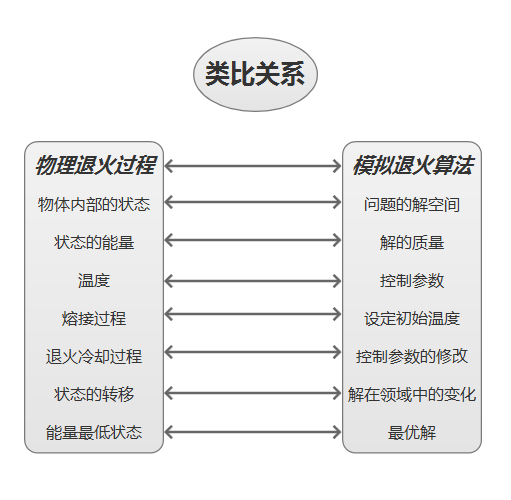
\includegraphics[width=0.7\linewidth]{模拟退火算法类比图}
		\caption{模拟退火算法与固体退火过程类比图}
		\label{fig:}
	\end{figure}
	
	
	
	
	\fontsize{14pt}{24pt}\textbf{\begin{flushleft}
			4.2模拟退火算法TSP模型的建立
	\end{flushleft}}
	\fontsize{12pt}{24pt}
	模型可以分为以下5步:
	
	1.构造TSP问题的解空间和初始解
	
	TSP问题的解空间S是一个遍历所有城市且每个城市仅经过一次的所有的回路,是所有城市排列的集合。TSP问题的解空间S可表示为{1,2,...,n}的全排列组合,即
	$$S=\{(c_{1},c_{2},...,c_{n})|(c_{1},c_{2},...,c_{n})\}$$
	其中$\S_{i}$表示遍历n个城市的一个路径,$\c_{i}=j$表示第i次访问城市j。由于该算法的解的质量对初始状态依赖性较弱,故初始解为随机函数生成一个\{1,2,...,n\}的随机排列作为$\S_{0}$
	
	2.构建目标函数
	
	TSP问题的目标函数即为遍历所有城市的路径总长度,即
	$$C(c_{1},c_{2},...,c_{n})=\sum_{i=1}^{n+1}d*(c_{i},c_{i+1})+d*(c_{1},c_{n})$$
	我们的目的为求解上式的最小值,则当上式最小时的城市排列即为所求的最短路径。
	
	3.产生新解
	
	新解的产生可以通过以下2种方法分别使用或者交替使用产生:
	
	二变换法:任选序号u、v(设u<v<n),交换u与v之间的访问顺序。
	
	三变换法:任选序号u、v(设u<v<n),u,v,w(设u<v<w)将u与v的路径插到w之后访问。
	
	4.目标函数差
	
	计算变换前的解和变换后的目标函数的差值:
	$$\Delta \acute{C}=C(\acute{s_{i}})-C(s_{i})$$
	
	5.Metropolis接受准则
	
	以新解与当前解的目标函数之差定义接受概率,即
	$$P=
	\left\{
	\begin{aligned}
	& 1,\acute{C}<0\\
	& \exp(-\Delta \acute{C}/T),\acute{C}>0
	\end{aligned}
	\right.
	$$	
	
	\fontsize{14pt}{24pt}\textbf{\begin{flushleft}
			4.3matlab实现模拟退火—TSP模型的具体操作
	\end{flushleft}}
	
	\fontsize{12pt}{24pt}
	首先,初始化温度衰减函数的参数,设定markov链程度为10000(即最大迭代次数为10000),并且读取城市坐标,记录到矩阵coordinates中。amount表示城市的数量。将初始解设置为1到amount的排列,记为$sol_new$。
	
	其次,计算每2个城市之间相邻的距离,并且将其保存到矩阵$dist_matrix$中。
	
	随后,进行随机扰动。采用while循环,当温度高于终止温度,循环进行一下操作:采用for循环,当迭代次数小于markov,则等可能地对当前解进行二交换或三交换产生新解$sol_new$。并对比新解与旧解的内能(目标函数值)的大小。若新解的内能更小,则将新解赋值给当前解,若当前解的内能更小,则仅以一定的概率接受新解。
	
	每当循环达到迭代次数,即上述for循环完成一次,则降低温度值t,模拟退火的降温过程。当t降至终止温度tf时,跳出while循环。
	
	最后,输出程序运行时间、最优解以及最短距离。
	
	
	
	
	
	\fontsize{14pt}{24pt}\textbf{\begin{flushleft}
			4.4对模拟退火算法求解结果的展示与分析
	\end{flushleft}}
	\fontsize{12pt}{24pt}matlab命令窗口输出结果为:
	
	程序执行时间:15.884秒
	
	最优解为:
	
	1 至 15 列
	
	18  { }   3   { } 17  { }  21 { }   42 { }    7  { }   2 { }   30  { }  23   { } 20  { }  50  { }  29  { }  16  { }  46  { }  44
	
	16 至 30 列
	
	34  { }  35  { }  36   { } 39  { }  40 { }   37  { }  38 { }   48  { }  24  { }   5  { }  15  { }   6 { }    4 { }   25  { }  12{ }
	
	31 至 45 列
	
	28  { }  27{ }    26  { }  47    { }13 { }   14{ }    52{ }    11 { }   51{ }    33 { }   43  { }  10 { }    9    { } 8 { }   41
	
	46 至 52 列
	
	19   { } 45   { } 32   { } 49     { }1   { } 22   { } 31
	
	最短距离:
	
	7.5444e+03
	
	最短路径的图像如下所示:
	\begin{figure}[H]
		\centering
		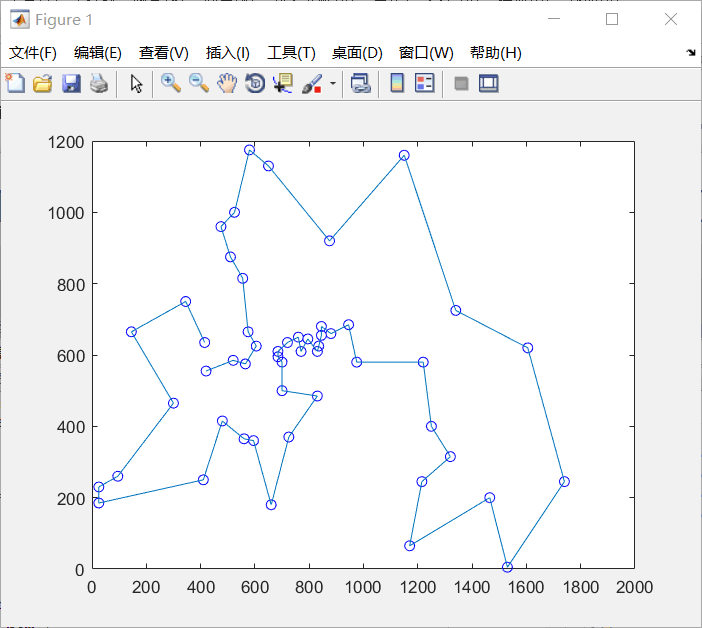
\includegraphics[width=0.7\linewidth]{模拟退火算法最优化路径}
		\caption{模拟退火算法最优化路径}
		\label{fig:}
	\end{figure}

反复多次运行同样的代码,所得的最短路径长度分别为7.5444e+03,7.6758e+03,7.5444e+03,所耗费的运行时间分别为19.031秒,18.15秒,18.769秒
	
	 分析可知:模拟退火算法的特点如下:
	 
	 优点为:
	 
	 1.局部搜索能力强。
	 
	 2.运行效率高,运行时间较短。
	 
	 缺点为:
	 
	 1.全局搜索能力差。
	 
	 2.容易受参数的影响。 
	
	\newpage
	
	\fontsize{14pt}{24pt}\textbf{\begin{center}
			五、MATLAB使用遗传算法解TSP问题
	\end{center} }
	
		\fontsize{14pt}{24pt}\textbf{\begin{flushleft}
			5.1遗传算法的原理
	\end{flushleft}}
	\fontsize{12pt}{24pt} 遗传算法基于生物学上的自然选择和基因遗传学原理,借鉴了优胜劣汰的自然选择机理和生物界繁衍进化的基因重组、突变的遗传机制,是一种全局自适应概率搜索算法。
	
	遗传算法通常的实现方式为一种计算机模拟。对于最优化问题,一定数量的候选解(即个体)可抽象表示为染色体,使种群向更优的解进化。进化从完全随机个体的种群开始,逐代繁衍下去。在每一代中评价整个种群的适应度,从当前种群中随机地选择多个个体,基于它们的适应度大小,通过自然选择和突变的方式产生新的生命种群,这些种群在算法的下一次迭代中成为当前种群。
	
	
	

	

	
	\fontsize{14pt}{24pt}\textbf{\begin{flushleft}
			5.2matlab实现遗传算法—TSP模型的具体操作
	\end{flushleft}}
	
	\fontsize{12pt}{24pt}
	1.构造初始化填充函数$create\_permutations$,创建交叉子集的函数$crossover\_permutation$,产生变异后代的函数$mutate\_permutation$,以及用于绘制由算法计算的数据的函数$my\_plot$。
	
	2.加载问题的数据与作图:
	
	读入文件points中的点的坐标,并将城市的横坐标x与纵坐标y绘制成二维直角图。
	
	3.计算点之间的距离:
	
	使用2个for循环,依次计算出每2个城市之间的距离大小,并记录在pointdis矩阵中,便于后续的计算。
	
	4.定义目标函数$points\_fitness$,用于求解适应度。
	
	5.设置优化属性并执行遗传算法求解
	
	
	
	
	
	
	\fontsize{14pt}{24pt}\textbf{\begin{flushleft}
			5.3遗传算法求解结果的展示与分析
	\end{flushleft}}
	\fontsize{12pt}{24pt}运行代码后,MATLAB命令行输出以下内容:
	
	Optimization terminated: average change in the fitness value less than options.FunctionTolerance.
	
	x =
	
	1×1 cell 数组
	
	{1×52 double}
	
	
	fval =
	
	8.1829e+03
	
	
	reason =
	
	1
	
	
	output = 
	
	包含以下字段的 struct:
	
	problemtype: 'unconstrained'
	
	rngstate: [1×1 struct]
	
	generations: 734
	
	funccount: 73500
	
	message: 'Optimization terminated: average change in the fitness value less than options.FunctionTolerance.'
	maxconstraint: []
	
	
	程序执行时间:54.802秒

	此时超过MAX { }STALL{ } GENERATION 后不再遗传变异,视为遗传终止
	。此时,图像窗口的最终形态为下图:\begin{figure}[H]
		\centering
		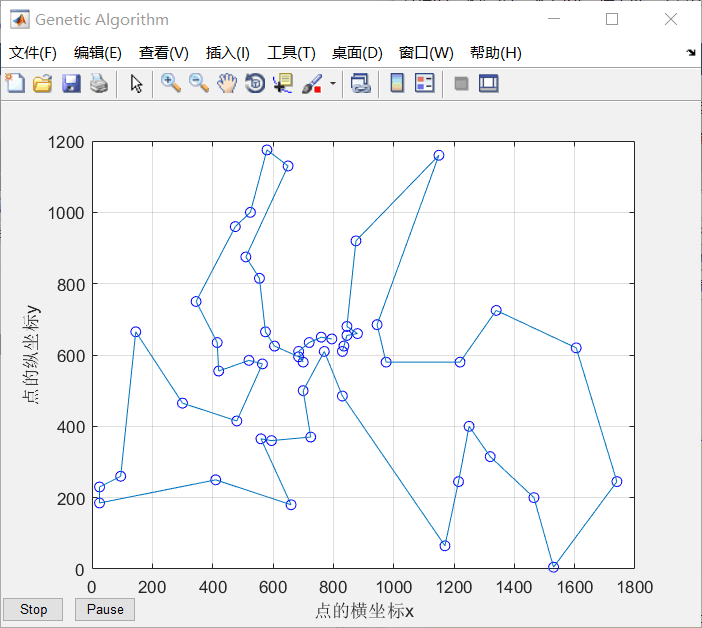
\includegraphics[width=0.7\linewidth]{遗传算法最优化路径}
		\caption{}
		\label{fig:}
	\end{figure}
	
     反复运行该程序,得到的运行时间分别为54.802秒,66.603秒,52.968秒,目标函数值分别为 8.1829e+03,8.1948e+03, 8.5765e+03。说明它的求解稳定性一般,且运行时间多于其他2种matlab算法,解的质量也显著低于其他2种算法。经过分析知:遗传算法每次终止条件都是达到最大代数,因此最大代数对运行时间以及解的质量有着较大的影响
	
	
	遗传算法在该问题中表现了以下特点:
	
	1.同时处理群体中的多个个体,即对搜索空间中的多个解进行评估,减少了陷入局部最优解的风险,同时算法本身易于实现并行化。
	
	2.具有自组织、自适应和自学习性。遗传算法利用进化过程获得的信息自行组织搜索时,适应度大的个体具有较高的生存概率,并获得更适应环境的基因结构。
	
	3.从问题解的串集开始搜索,而不是从单个解开始。这是遗传算法与传统优化算法的极大区别。传统优化算法是从单个初始值迭代求最优解的;容易误入局部最优解。遗传算法从串集开始搜索,覆盖面大,利于全局择优。
	\newpage
	
	
	\fontsize{14pt}{24pt}\textbf{\begin{center}
			六、lingo解TSP问题
	\end{center} }
	\fontsize{14pt}{24pt}\textbf{\begin{flushleft}
			6.1lingo的特点与优势
	\end{flushleft}	}
	\fontsize{12pt}{24pt}  
	\begin{flushleft}
	(1)既能求解线性规划问题,也有较强的求解非线性规划问题的能力;
	
	
	(2)输入模型简练直观;
	
	(3)运行速度快,计算能力强;
	
	(4)内置建模语言,提供几十个内部函数,从而能以较少语句,较直观的方式描述较大规模的优化模型;
	
	(5)将集合的概念引入编程语言,很容易将实际问题转换为LINGO模型;
	
	(6)能方便地与Excel、数据库等其他软件交换数据;
	\end{flushleft}


	\fontsize{14pt}{24pt}\textbf{\begin{flushleft}
			6.2lingo-TSP模型的建立
	\end{flushleft}	}
	\fontsize{12pt}{24pt} 
	由于lingo没有可视化的功能,我们不能直观地将路线图表示出来,因此不再需要将每个点的坐标进行表示,而是直接应用每两个城市间的距离直接进行计算。为了简化模型,我们使用matlab计算出所有的相邻2个城市之间的距离并输出一个Excel表格,将表格中的数据复制到lingo的数据输入部分。
	
	假使每次路线的起点与终点相同,则路线为一条闭合的回路。则无论起点为52个城市中的哪一个,所求得的路线均为相同的。我们不妨假设起点城市的序号即为1。
	
	
	\fontsize{14pt}{24pt}\textbf{\begin{flushleft}
			6.3lingo编程与模型结合的思路
	\end{flushleft}	}
	\fontsize{12pt}{24pt} 
	一般而言,lingo编程解题可以分为一下四步:
	
	1.在集合段声明变量:
	
	声明名为city的集合,集成员为1到52的整数。其中num为city的集属性,用来表示52个不同的城市。
	
	声明名为link的派生集,它由2个city派生而成,dist与x为link的集属性。其中dist为距离矩阵,dist(i,j)表示城市i与城市j之间的距离。x为路线矩阵,x(i,j)=0表示在求解的路线中城市i与城市j之间不相连,x(i,j)=1表示在求解的路线中城市i与城市j之间不相连。
	
	2.在数据段输入解题所必需的数据:
	
	
	
	
	3.在初始段输入初始条件:
	
	由于我们已经假设每次路线的起点与终点相同,则路线为一条闭合的回路。则无论起点为52个城市中的哪一个,所求得的路线均为相同的。我们不妨假设起点城市的序号即为1。因此这个环节在我们对TSP问题的求解中不必要。
	
	4.在目标与约束段输入目标函数和约束条件:
	
	由模型可知,我们的目标函数即为路线的总距离,它可以用距离矩阵和路线矩阵相同位置的项的乘积来进行表示。我们可以使用lingo自带的min函数对其进行求解。
	
	而约束条件有三个。首先由于每次选择的路线的唯一性,我们可以知道,每一个城市i之前,有且仅有一个城市j与其相连。相应的,每一个城市j之后,有且仅有一个城市i与其相连。我们可以用集循环函数对这两个约束条件进行描述。
	
	第三个条件是最为关键,也最容易忽略的一个。若城市i与城市j相邻,则x(i,j)=1,且num(i)-num(j)=-1,则恰好使得num(i)-num(j)+52*x(i,j)<=51的等号成立,
	若城市i与城市j不相邻,则x(i,j)=0,且num(i)-num(j)的最大值为51,同样满足此式的等号成立。这样就有效的限制了路线是一个由52个城市组成的且不重复经过任何一个城市的闭合回路。
	
	
	\fontsize{14pt}{24pt}\textbf{\begin{flushleft}
		6.4对lingo解答的结果分析
\end{flushleft}	}
\fontsize{12pt}{24pt} 	
	lingo自带的运行状态窗口如下图:
	\begin{figure}[H]
		\centering
		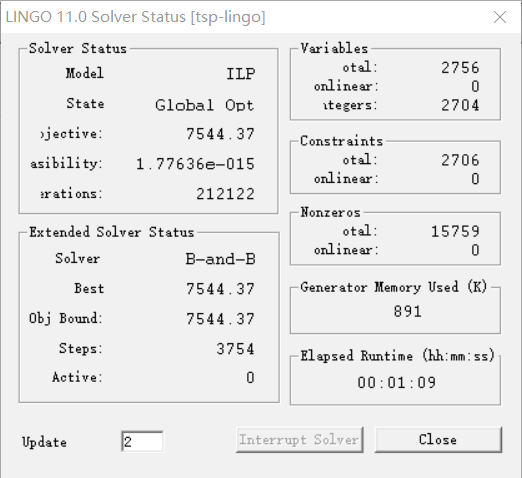
\includegraphics[width=0.7\linewidth]{lingo报告}
		\caption{lingo运行状态窗口}
		\label{fig:lingo}
	\end{figure}
	
	
	由上可知:TSP为整数线性规划问题,该模型共2756个变量,其中2704个为整数变量。约束条件有2706个,全为线性约束。非零的系数有15759个。目标函数的最小值为7544.37.lingo采用的是B-B求解器(分枝定界算法)。值得注意的是,其运行时间较长,比matlab3种算法所耗费的时间均要长。这直观地证明了matlab对求解TSP问题的效率之高。
	
	反复多次运行lingo程序,得到的目标函数值稳定不变,而运行时间分别为1分09秒,1分17秒,1分10秒。这证明了lingo求解的稳定性是比较高的。
	
	将第三个之前提到的第三个约束条件删去,得到的目标函数的值为6285.96,小于有约束条件时的目标函数值7544.37,且运行时间仅需1秒。由此可知第三个约束是紧约束,是不可缺少的关键约束条件。
	

	
	\fontsize{12pt}{24pt} 
	对比上面四种解题方法,我们可以发现:使用lingo进行求解是在描述模型上面最直观。使用lingo可以避免复杂繁琐的函数,而直接用内置的min函数即可自动选取合适的求解器有针对性地实现解答。它的解的精确度也是最高的。但是它的缺点在于求解效率显著低于matlab的算法,且不能将每个城市的坐标以及具体路线进行可视化。
	
	\newpage
		\fontsize{14pt}{24pt}\textbf{\begin{center}
			七、对比总结
	\end{center} } 	
	
	
	\fontsize{12pt}{24pt}
	由于我们对每种算法采用了相同的城市坐标数据,我们很容易能将4种方法进行比对分析。经过分析,我们得到以下结论:
	
	1.lingo是4种方法里面最容易描述TSP问题的。它仅需输入数据、约束条件以及目标函数,即可自动选择合适的求解器。对于TSP问题,它采用了B—and—B求解器,即分枝定界算法。lingo求得的目标函数值最为精确。而lingo相比matlab的缺陷在于,它的运行时间较长,显著多于matlab的算法,在运行效率上有着较大的劣势。而且它不能实现最短路径的可视化,在描述运算结果方面不如matlab直观。
	
	2.lingo的求解稳定性是4者当中最优的。多次重复运行同样的代码,所得的计算结果以及运行所用时间均无明显变化。
	
	3.不论采取何种算法,matlab相比lingo,都有着可以实现城市位置以及具体线路的可视化的优势,这使得计算结果更加直观。
	
	4.模拟退火算法是matlab3种算法计算效率最高的,计算结果也略优于其他几个算法,这证明了模拟退火算法的可靠性与有效性。
	
	
	5.蚁群算法的运行速度仅次于模拟退火算法,但是它的解的质量不如模拟退火算法和lingo的。
	
	6.遗传算法的运行时间是3种matlab算法中最长的,且解的质量是4种方法里面最低的。这说明代码尚有较大的优化空间。
	
	7.综上可知,我们讨论的4种方法中,对TSP问题适应性最好的是模拟退火算法,其次是lingo。最需要改进的是遗传算法。
	
	
	
	\newpage
	
	
	\fontsize{14pt}{24pt}\textbf{\begin{center}
			八、4种方法可能改进的方向
	\end{center} } 	
		\fontsize{14pt}{24pt}\textbf{\begin{flushleft}
			8.1蚁群算法的可能改进方向
	\end{flushleft}	}
	\fontsize{12pt}{24pt}  
\begin{flushleft}
		1.蚂蚁数量m可以多次修改,并对比各种不同m下程序的运行时间与解的质量,以求得更为合适的参数值。分析可知:当m过大,会导致路径上的信息素量变化趋于平均,正反馈作用减弱,导致收敛速度减慢。当m过小,可能使程序过早停滞,以致于解的全局优化性降低。
	
	2.若信息素因子的值过大,则蚂蚁选择已经走过的路径的概率会过更大,搜索的随机性就会减弱;若过小,则等同于贪婪算法,使搜索过早陷入局部最优。
	
	3.若启发函数因子过大,会使搜索速度提高,但是搜索全局最优解的随机性会减弱,易于陷入局部最优。若值过小,则群体会陷入纯粹的随机搜索,难以找到最优解。
	
	4.信息素挥发因子的值过大,则可能会重复搜索,若过小,则会减慢收敛速度。
	
	5.信息素常数的值若过大收敛速度加快,但是易于陷入局优。若过小,则运行速率会减慢。
	
	6.最大迭代次数过大,会浪费时间,可能在达到最大迭代次数前就已经收敛。若过小,则可能来不及收敛
\end{flushleft}
	
	
	
		\fontsize{14pt}{24pt}\textbf{\begin{flushleft}
			8.2模拟退火算法的可能改进方向
	\end{flushleft}	}
	\fontsize{12pt}{24pt}
	1.初始温度应该足够高。若温度不够高,则可能退火过程终止过快。若温度过高,则算法收敛速度会减慢。因此我们应反复调节初始温度,选择最合适的值。
	
	2.终止温度与初始温度同理。应当反复调参,确保参数的合理性。
	
	3.markov链长度应当合理。迭代次数不宜过多或过少。
	
	4.metropolis准则中的接受函数的参数k也应当取一个适应各个具体问题的值。
	
	
	
		\fontsize{14pt}{24pt}\textbf{\begin{flushleft}
			8.3遗传算法的可能改进方向
	\end{flushleft}	}
	\fontsize{12pt}{24pt}
	分析可知,遗传算法的函数ga是matlab内置的函数,可以用控制变量测试一下参数如何设置得出来的解最优。又测试知:遗传算法在3种算法中运行时间最长,且解的质量是4种方法中最低的。因此遗传算法在TSP问题的代码上还有较大的优化空间。
	
		\fontsize{14pt}{24pt}\textbf{\begin{flushleft}
			8.4lingo代码的可能改进方向
	\end{flushleft}	}
	\fontsize{12pt}{24pt}
	分析可知:整个lingo代码仅有输入数据、表示目标函数、表示约束条件三个部分,而求解器是由lingo自动选择,其求解速度和解的质量由lingo本身所决定,故lingo代码在提高运行速度和解的质量方面的优化还有待进一步的研究。
	\newpage
	
	\fontsize{14pt}{24pt}\textbf{\begin{center}
			九、参考文献
	\end{center} } 	
	
	\begin{flushleft}
		[1] 卓金武 {  }王鸿钧.MATLAB数学建模方法与实践[M].3.北京航天航空大学, 2018.
	\end{flushleft}
	
	\newpage
	
	
	
	\fontsize{14pt}{24pt}\textbf{\begin{center}
			附录
	\end{center} }
	\fontsize{14pt}{24pt}\begin{flushleft}
		\textbf{1.MATLAB使用蚁群算法解TSP问题的代码}
	\end{flushleft}
	\fontsize{12pt}{24pt}
	
	\lstset{language=matlab}
	\begin{lstlisting}
		clear all
	clc
	
	
	t0 = clock;
	
	points=xlsread('points_data.xlsx', 'B2:C53');
	
	
	n = size(points,1);
	D = zeros(n,n);
	for i = 1:n
	for j = 1:n
	if i ~= j
	D(i,j) = sqrt(sum((points(i,:) - points(j,:)).^2));
	else
	D(i,j) = 1e-4;      
	end
	end    
	end
	
	m = 75;                             
	alpha = 1;                          
	beta = 5;                          
	vol = 0.2;                          
	Q = 10;                             
	Heu_F = 1./D;                       
	Tau = ones(n,n);                    
	Table = zeros(m,n);                
	iter = 1;                           
	iter_max = 100;                     
	Route_best = zeros(iter_max,n);     
	Length_best = zeros(iter_max,1);      
	Length_ave = zeros(iter_max,1);      
	Limit_iter = 0;                   
	
	while iter <= iter_max
	
	start = zeros(m,1);
	for i = 1:m
	temp = randperm(n);
	start(i) = temp(1);
	end
	Table(:,1) = start; 
	
	points_index = 1:n;
	
	for i = 1:m
	
	for j = 2:n
	tabu = Table(i,1:(j - 1));         
	allow_index = ~ismember(points_index,tabu);  
	allow = points_index(allow_index);  
	P = allow;
	
	for k = 1:length(allow)
	P(k) = Tau(tabu(end),allow(k))^alpha * Heu_F(tabu(end),allow(k))^beta;
	end
	P = P/sum(P);
	
	Pc = cumsum(P);   
	target_index = find(Pc >= rand);   
	target = allow(target_index(1));   
	Table(i,j) = target;
	end
	end
	
	Length = zeros(m,1);
	for i = 1:m
	Route = Table(i,:);
	for j = 1:(n - 1)
	Length(i) = Length(i) + D(Route(j),Route(j + 1));
	end
	Length(i) = Length(i) + D(Route(n),Route(1));
	end
	
	if iter == 1
	[min_Length,min_index] = min(Length);
	Length_best(iter) = min_Length;  
	Length_ave(iter) = mean(Length);
	Route_best(iter,:) = Table(min_index,:);
	Limit_iter = 1; 
	
	else
	[min_Length,min_index] = min(Length);
	Length_best(iter) = min(Length_best(iter - 1),min_Length);
	Length_ave(iter) = mean(Length);
	if Length_best(iter) == min_Length
	Route_best(iter,:) = Table(min_index,:);
	Limit_iter = iter; 
	else
	Route_best(iter,:) = Route_best((iter-1),:);
	end
	end

	Delta_Tau = zeros(n,n);

	for i = 1:m

	for j = 1:(n - 1)
	Delta_Tau(Table(i,j),Table(i,j+1)) = Delta_Tau(Table(i,j),Table(i,j+1)) + Q/Length(i);
	end
	Delta_Tau(Table(i,n),Table(i,1)) = Delta_Tau(Table(i,n),Table(i,1)) + Q/Length(i);
	end
	Tau = (1-vol) * Tau + Delta_Tau;
	
	iter = iter + 1;
	Table = zeros(m,n);
	end
	
	
	[Shortest_Length,index] = min(Length_best);
	Shortest_Route = Route_best(index,:);
	Time_Cost=etime(clock,t0);
	disp(['最短距离:' num2str(Shortest_Length)]);
	disp(['最短路径:' num2str([Shortest_Route Shortest_Route(1)])]);
	disp(['收敛迭代次数:' num2str(Limit_iter)]);
	disp(['程序执行时间:' num2str(Time_Cost) '秒']);
	
	figure(1)
	plot([points(Shortest_Route,1);points(Shortest_Route(1),1)],...  
	[points(Shortest_Route,2);points(Shortest_Route(1),2)],'o-');
	grid on
	for i = 1:size(points,1)
	text(points(i,1),points(i,2),['   ' num2str(i)]);
	end
	text(points(Shortest_Route(1),1),points(Shortest_Route(1),2),'       起点');
	text(points(Shortest_Route(end),1),points(Shortest_Route(end),2),'       终点');
	xlabel('点位置横坐标')
	ylabel('点位置纵坐标')
	title(['ACA最优化路径(最短距离:' num2str(Shortest_Length) ')'])
	figure(2)
	plot(1:iter_max,Length_best,'b')
	legend('最短距离')
	xlabel('迭代次数')
	ylabel('距离')
	title('算法收敛轨迹')
	
	
	
	\end{lstlisting}
	
	\fontsize{14pt}{24pt}\begin{flushleft}
		\textbf{2.MATLAB使用模拟退火算法解TSP问题的代码}
	\end{flushleft}
	\fontsize{12pt}{24pt} 
	\lstset{language=C}
	\begin{lstlisting}
	
	clear all,clc
	ttt=clock;
	a = 0.99;
	t0 = 97; tf = 3; t = t0;
	Markov_length = 10000;	
	points = xlsread('points_data.xlsx', 'B2:C53');
	numofpoi = size(points,1); 

	pointsidis = zeros(numofpoi, numofpoi);
	coor_x_tmp1 = points(:,1) * ones(1,numofpoi);
	coor_x_tmp2 = coor_x_tmp1';
	coor_y_tmp1 = points(:,2) * ones(1,numofpoi);
	coor_y_tmp2 = coor_y_tmp1';
	pointsidis = sqrt((coor_x_tmp1-coor_x_tmp2).^2 + ...
	(coor_y_tmp1-coor_y_tmp2).^2);
	
	sol_new = 1:numofpoi;        

	E_current = inf;E_best = inf; 
	sol_current = sol_new; sol_best = sol_new;          
	p = 1;
	
	while t>=tf
	for r=1:Markov_length	
	if (rand < 0.5)
	ind1 = 0; ind2 = 0;
	while (ind1 == ind2)
	ind1 = ceil(rand.*numofpoi);
	ind2 = ceil(rand.*numofpoi);
	end
	tmp1 = sol_new(ind1);
	sol_new(ind1) = sol_new(ind2);
	sol_new(ind2) = tmp1;
	else

	ind1 = 0; ind2 = 0; ind3 = 0;
	while (ind1 == ind2) || (ind1 == ind3) ...
	|| (ind2 == ind3) || (abs(ind1-ind2) == 1)
	ind1 = ceil(rand.*numofpoi);
	ind2 = ceil(rand.*numofpoi);
	ind3 = ceil(rand.*numofpoi);
	end
	tmp1 = ind1;tmp2 = ind2;tmp3 = ind3;

	if (ind1 < ind2) && (ind2 < ind3)
	;
	elseif (ind1 < ind3) && (ind3 < ind2)
	ind2 = tmp3;ind3 = tmp2;
	elseif (ind2 < ind1) && (ind1 < ind3)
	ind1 = tmp2;ind2 = tmp1;
	elseif (ind2 < ind3) && (ind3 < ind1) 
	ind1 = tmp2;ind2 = tmp3; ind3 = tmp1;
	elseif (ind3 < ind1) && (ind1 < ind2)
	ind1 = tmp3;ind2 = tmp1; ind3 = tmp2;
	elseif (ind3 < ind2) && (ind2 < ind1)
	ind1 = tmp3;ind2 = tmp2; ind3 = tmp1;
	end
	
	tmplist1 = sol_new((ind1+1):(ind2-1));
	sol_new((ind1+1):(ind1+ind3-ind2+1)) = ...
	sol_new((ind2):(ind3));
	sol_new((ind1+ind3-ind2+2):ind3) = ...
	tmplist1;
	end

	

	E_new = 0;
	for i = 1 : (numofpoi-1)
	E_new = E_new + ...
	pointsidis(sol_new(i),sol_new(i+1));
	end
	
	E_new = E_new + ...
	pointsidis(sol_new(numofpoi),sol_new(1));
	
	if E_new < E_current
	E_current = E_new;
	sol_current = sol_new;
	if E_new < E_best
	
	E_best = E_new;
	sol_best = sol_new;
	end
	else

	if rand < exp(-(E_new-E_current)./t)
	E_current = E_new;
	sol_current = sol_new;
	else	
	sol_new = sol_current;
	end
	end
	end
	t=t.*a;		
	end
	
	Time_Cost=etime(clock,ttt);
	disp(['程序执行时间:' num2str(Time_Cost) '秒']); 
	disp('最优解为:')
	disp(sol_best)
	disp('最短距离:')
	disp(E_best)
	plot(points(:,1),points(:,2),'bo')
	axis([0 2000 0 1200]);
	hold on
	plot(points(sol_best,1),points(sol_best,2))
	
	
	
	\end{lstlisting}
	
	\fontsize{14pt}{24pt}\begin{flushleft}
		\textbf{3.1MATLAB使用遗传算法解TSP问题的主代码}
	\end{flushleft}
	\fontsize{12pt}{24pt} 
	\lstset{language=matlab}
	\begin{lstlisting}


	 ttt=clock;
	 points =xlsread('points_data.xlsx', 'B2:C53');
	 numofpo=size(points,1);
	 plot(points(:,1),points(:,2),'bo');
	 xlabel('点的横坐标x'); ylabel('点的纵坐标y'); 
	 grid on
	 

	 
	 pointdis = zeros(numofpo);
	 for count1=1:numofpo
	 for count2=1:count1
	 x1 = points(count1,1);
	 y1 = points(count1,2);
	 x2 = points(count2,1);
	 y2 = points(count2,2);
	 pointdis(count1,count2)=sqrt((x1-x2)^2+(y1-y2)^2);
	 pointdis(count2,count1)=pointdis(count1,count2);
	 end
	 end
	 
	 

	 FitnessFcn = @(x) points_fitness(x,pointdis); 
	 
	 my_plot = @(options,state,flag) points_plot(options, ...
	 state,flag,points);
	 

	 
	 options = optimoptions(@ga, 'PopulationType', 'custom','InitialPopulationRange', ...
	 [1;numofpo]);      
	 
	 options = optimoptions(options,'CreationFcn',@create_permutations, ... 
	 'CrossoverFcn',@crossover_permutation, ...     
	 'MutationFcn',@mutate_permutation, ...        
	 'PlotFcn', my_plot, ...                      
	 'MaxGenerations',1000,'PopulationSize',100, ...  
	 'MaxStallGenerations',200,'UseVectorized',true);
	 
	 numberOfVariables = numofpo;
	 [x,fval,reason,output] = ...
	 ga(FitnessFcn,numberOfVariables,[],[],[],[],[],[],[],options)
	 Time_Cost=etime(clock,ttt);
	 disp(['程序执行时间:' num2str(Time_Cost) '秒']); 
	 
	
	\end{lstlisting}
	
	\fontsize{14pt}{24pt}\begin{flushleft}
		\textbf{3.2create$\_$permutations函数的代码}
	\end{flushleft}
	\fontsize{12pt}{24pt} 
	\lstset{language=matlab}
	\begin{lstlisting}
	function pop = create_permutations(NVARS,FitnessFcn,options)
	
	totalPopulationSize = sum(options.PopulationSize);
	n = NVARS;
	pop = cell(totalPopulationSize,1);
	for i = 1:totalPopulationSize
	pop{i} = randperm(n); 
	end
	
	\end{lstlisting}
	
	\fontsize{14pt}{24pt}\begin{flushleft}
		\textbf{3.3crossover$\_$permutations函数的代码}
	\end{flushleft}
	\fontsize{12pt}{24pt} 
	\lstset{language=matlab}
	\begin{lstlisting}
function xoverKids  = crossover_permutation(parents,options,NVARS, ...
FitnessFcn,thisScore,thisPopulation)


nKids = length(parents)/2;
xoverKids = cell(nKids,1);

for i=1:nKids

parent = thisPopulation{parents(index)};
index = index + 2;


p1 = ceil((length(parent) -1) * rand);
p2 = p1 + ceil((length(parent) - p1- 1) * rand);
child = parent;
child(p1:p2) = fliplr(child(p1:p2));
xoverKids{i} = child;
end

	\end{lstlisting}
	
	\fontsize{14pt}{24pt}\begin{flushleft}
		\textbf{3.4mutate$\_$permutations函数的代码}
	\end{flushleft}
	\fontsize{12pt}{24pt} 
	\lstset{language=matlab}
	\begin{lstlisting}
	function mutationChildren = mutate_permutation(parents ,options,NVARS, ...
	FitnessFcn, state, thisScore,thisPopulation,mutationRate)

	mutationChildren = cell(length(parents),1);
	for i=1:length(parents)
	parent = thisPopulation{parents(i)};
	p = ceil(length(parent) * rand(1,2));
	child = parent;
	child(p(1)) = parent(p(2));
	child(p(2)) = parent(p(1));
	mutationChildren{i} = child;
	end
	
	
	\end{lstlisting}
	
	
	\fontsize{14pt}{24pt}\begin{flushleft}
		\textbf{3.5points$\_$fitness函数的代码}
	\end{flushleft}
	\fontsize{12pt}{24pt} 
	\lstset{language=matlab}
	\begin{lstlisting}
	function scores = points_fitness(x,distances)
	scores = zeros(size(x,1),1);
	for j = 1:size(x,1)
	p = x{j}; 
	f = distances(p(end),p(1));
	for i = 2:length(p)
	f = f + distances(p(i-1),p(i));
	end
	scores(j) = f;
	end
	
	\end{lstlisting}
	
	\fontsize{14pt}{24pt}\begin{flushleft}
		\textbf{3.6points$\_$plot函数的代码}
	\end{flushleft}
	\fontsize{12pt}{24pt} 
	\lstset{language=matlab}
	\begin{lstlisting}
	function state = points_plot(options,state,flag,points)
	if strcmpi(flag,'init')
	points =xlsread('points_data.xlsx', 'B2:C53');
	end
	[~,i] = min(state.Score);
	genotype = state.Population{i};
	
	plot(points(:,1),points(:,2),'bo');
	
	hold on
	plot(points(genotype,1),points(genotype,2));
	xlabel('点的横坐标x'); ylabel('点的纵坐标y'); 
	grid on
	hold off
	
	\end{lstlisting}
	
	\fontsize{14pt}{24pt}\begin{flushleft}
		\textbf{4.lingo解TSP问题的代码}
	\end{flushleft}
	\fontsize{12pt}{24pt} 
	\lstset{language=lingo}
	\begin{lstlisting}
	
	model:
	sets:
	city/1..52/:num;
	link(city,city):dist,x;

	endsets
	
	data:
	dist=
	0	666.1080993	281.1138559	395.6008089	291.2043956	326.266762	640.8002809	426.8782028	600.1874707	561.4712815	1040.973102	655.0190837	975	1120.769825	299.0401311	260.0480725	429.5346319	161.5549442	305	210.0595154	286.9233347	46.09772229	181.1767093	274.5906044	410.0304867	728.9718787	798.5142453	707.0007072	406.2634613	360.0694377	146.3728117	90.55385138	827.314934	135.0925609	121.6552506	125	207.9663434	240.4163056	166.2077014	208.9258242	395.3795645	565.7958996	463.8156962	154.4344521	240.208243	279.8660394	791.2806076	267.3013281	64.03124237	217.0829335	789.3826702	1220.460978
	666.1080993	0	649.3265742	1047.091209	945.1454914	978.0848634	45	956.1511387	1134.955946	1132.982789	1638.787662	1258.590481	1440.078123	1515.725899	957.8230526	724.033839	494.7726751	595.4829972	843.4008537	564.4687768	392.4601891	636.4157446	509.8284025	921.7917335	1028.846441	1191.511645	1301.50874	1243.724246	635.0196847	390.4484601	541.2254613	730	1488.707493	782.0805585	776.9813383	785	857.7004139	896.9392399	827.9643712	869.7413409	896.1724164	102.5914226	1123.710372	744.8825411	823.2860985	859.0838143	1151.271037	910.3021476	728.0109889	596.2591718	1421.557245	1716.049242
	281.1138559	649.3265742	0	603.5105633	508.9449872	542.5172808	610.5735009	308.058436	485.6439025	487.2627628	1266.688596	891.3613184	1247.757989	1399.732117	504.8762225	537.4011537	217.3131381	134.6291202	207.0024154	440.9648512	288.5307609	240.5202694	361.1786262	505.6925944	652.533524	1005.94483	1067.637579	970.3221115	651.2488004	504.2072986	208.9258242	245.2039967	903.3963693	393.6051321	373.6642878	367.6955262	447.4650824	462.087654	392.2371731	426.8782028	246.9817807	550.0909016	556.596802	434.1946568	219.8294794	552.6753116	1072.310589	504.8019414	288.4874347	463.2493929	995.3140208	1483.59361
	395.6008089	1047.091209	603.5105633	0	104.4030651	69.64194139	1026.364945	525	611.0032733	533.9007398	663.1930337	294.3637206	711.0731327	897.0089186	100.124922	384.2199891	800.2499609	532.3532662	474.6841055	500.6246099	681.487344	436.6062299	537.7034499	125.2996409	109.2016483	516.23638	526.8064161	417.4326293	579.8706752	689.5288246	540.8558033	370.5401463	517.3490118	266.5520587	275.1363298	270.6011826	190.3943276	155.241747	230.4886114	188.2817038	544.5410912	950.3288904	245.2039967	307.0016287	411.0960958	230.7054399	659.5642501	137.2953022	345.25353	477.6243294	397.0201506	908.6390923
	291.2043956	945.1454914	508.9449872	104.4030651	0	35.35533906	923.5935253	470.5581792	583.6308765	513.4685969	760.8054942	382.4264635	769.0416114	944.3119188	25	309.2329219	700.0714249	430.464865	400.7804885	406.6017708	577.169819	332.4530042	436.8352092	31.6227766	150.0833102	552.2680509	584.1446739	478.591684	509.754843	594.3483827	436.6062299	270.1851217	589.9576256	163.2482772	170.8800749	166.2077014	87.46427842	50.99019514	126.589889	85.14693183	479.5049531	847.6585397	266.6927071	212.2498528	331.2099032	170.6604817	673.5911223	47.4341649	241.8677324	386.684626	499.9249944	984.441466
	326.266762	978.0848634	542.5172808	69.64194139	35.35533906	0	957.0397066	491.5536593	596.0075503	523.2590181	726.1026098	349.2849839	744.1941951	922.7811225	40.31128874	328.8236609	735.0170066	465.6715581	427.9310692	435.2298243	611.9027701	367.7295202	469.0682253	57.00877125	124.1974235	533.3385416	559.1287866	452.2167622	528.0151513	623.6986452	471.8315377	305.0409809	568.2429058	196.977156	205.5480479	201.3082214	120.8304597	86.31338251	161.9413474	120.4159458	504.0089285	881.0363216	260.0480725	240.8318916	360.0694377	182.0027472	661.9101147	70.71067812	277.2183255	413.7934267	464.5696934	954.8952822
	640.8002809	45	610.5735009	1026.364945	923.5935253	957.0397066	0	918.0958556	1095.924267	1095.73035	1627.421273	1245.200787	1440.312466	1521.725994	935.3608929	713.8627319	451.2482687	562.2499444	807.0006196	551.7698796	361.731945	609.1387362	491.1720676	901.1797823	1012.422837	1190.094534	1297.786577	1236.739665	636.9654622	385.5191305	511.5173506	701.2310604	1459.631803	760.3453163	754.2048793	761.5773106	836.3163277	874.7142391	804.394182	846.5370636	857.554663	76.15773106	1094.805919	726.997249	789.3826702	844.4228798	1156.827558	890.1825655	701.7300051	584.6366393	1405.080069	1715.065596
	426.8782028	956.1511387	308.058436	525	470.5581792	491.5536593	918.0958556	0	183.4393633	180.346888	1144.901743	812.0498753	1234.34193	1414.23124	452.54834	660.9841148	506.5816815	381.2151623	125.8967831	635.9638354	580.3878014	415.0301194	586.7282165	486.5439343	615.5485359	1022.802522	1049.404593	941.0765112	831.0385069	758.7654447	457.2198596	338.7107911	645.1550201	455	435.4595274	421.5447782	460.5702987	446.0100896	413.8236339	421.57443	64.03124237	855.8621384	359.0264614	529.7405025	187.4166481	598.5398901	1135.89172	495.1009998	383.4383914	643.8167441	860.1453366	1430.47195
	600.1874707	1134.955946	485.6439025	611.0032733	583.6308765	596.0075503	1095.924267	183.4393633	0	83.21658489	1165.611428	873.8563955	1316.757381	1507.116452	561.4712815	817.9547665	670.3170891	564.6459067	308.058436	810.246876	763.2168761	593.0430001	766.5507159	606.238402	714.177849	1126.110563	1134.548368	1024.463274	998.2108996	940.4918926	640.3124237	510.0245092	570.1973343	606.9802303	589.4276885	574.6738205	596.0914359	571.9484242	557.8530272	555	239.2697223	1035.591618	389.9358922	685.5836929	360.8670115	733.8937253	1257.060062	617.8389758	550.5678886	815.1380251	883.2326987	1486.775033
	561.4712815	1132.982789	487.2627628	533.9007398	513.4685969	523.2590181	1095.73035	180.346888	83.21658489	0	1082.647219	792.0858539	1236.577939	1428.294437	490.4334817	763.6916917	686.4765109	547.9507277	290.9037642	770.2759246	751.4818694	560.2901034	734.9319696	537.8196724	638.846617	1049.97619	1055.047392	944.9338601	950.0526301	912.1403401	619.2939528	471.009554	500.8991915	552.2680509	536.1436375	521.1765536	533.6665626	506.2114183	499.9249944	492.4428901	243.977458	1031.952034	307.7742679	631.9810124	329.0136775	669.6454286	1185.168764	550.2726597	507.0009862	771.9617866	800.0781212	1404.038817
	1040.973102	1638.787662	1266.688596	663.1930337	760.8054942	726.1026098	1627.421273	1144.901743	1165.611428	1082.647219	0	387.0723447	442.7188724	619.5562928	762.3647421	914.8223871	1460.693329	1190.094534	1124.299782	1075.662587	1314.172744	1085.564369	1143.525251	770.0162336	631.2685641	541.0406639	417.4326293	417.6421914	1042.413066	1250.969624	1186.781361	1030.982541	706.13384	905.8835466	920.3396112	920.0543462	835.0598781	810.3857106	885.1271095	845.5323767	1180.042372	1552.320843	789.2401409	912.9211357	1067.953651	786.6701977	705.1595564	775.0645134	1000.0125	1042.928569	285.0438563	398.5599077
	655.0190837	1258.590481	891.3613184	294.3637206	382.4264635	349.2849839	1245.200787	812.0498753	873.8563955	792.0858539	387.0723447	0	452.1338297	653.2419154	388.1043674	537.7034499	1078.355229	806.8766944	768.8465387	694.1361538	927.1596411	700.0178569	758.172144	387.6209489	245	335.0373114	283.2401808	182.4828759	688.1860214	874.6427842	800.3905297	650.5766673	584.2088668	520	535.2102391	535.8404613	450.9988914	429.9418565	503.0159043	465.295605	836.3163277	1169.626009	484.3810483	526.1178575	705.301354	401.4037867	517.4214916	391.1521443	616.6441437	662.5896166	188.2153022	618.5668921
	975	1440.078123	1247.757989	711.0731327	769.0416114	744.1941951	1440.312466	1234.34193	1316.757381	1236.577939	442.7188724	452.1338297	0	205.5480479	784.0918314	759.2759709	1399.508842	1136.540804	1169.46569	919.9184746	1194.75939	1020.416582	1008.19145	759.9506563	620.0806399	254.0177159	185.0675552	293.6409372	805.2484089	1056.18417	1103.653025	1004.153873	1010.358847	854.1808942	874.3140168	881.192374	806.9231686	804.31648	862.6992523	836.3761116	1248.078523	1371.313239	930.8598176	821.7207555	1098.328275	696.0244249	324.422564	755.8604369	959.2835869	884.5903006	539.6758286	278.6574959
	1120.769825	1515.725899	1399.732117	897.0089186	944.3119188	922.7811225	1521.725994	1414.23124	1507.116452	1428.294437	619.5562928	653.2419154	205.5480479	0	961.6912186	883.8834765	1534.218042	1280.673651	1340.634178	1034.649699	1313.202193	1164.6888	1127.208942	931.3565375	799.1558046	396.0113635	374.4329045	484.1745553	887.4260533	1146.483755	1238.789732	1160.872517	1215.905013	1009.715306	1030.594489	1039.254541	971.4036236	974.5896572	1026.157883	1004.452587	1423.042515	1457.480703	1125.277743	966.3979512	1267.566566	848.763807	364.9657518	925.216191	1113.564098	1000.124992	744.6475676	318.9043744
	299.0401311	957.8230526	504.8762225	100.124922	25	40.31128874	935.3608929	452.54834	561.4712815	490.4334817	762.3647421	388.1043674	784.0918314	961.6912186	0	332.4154028	700.1606958	432.3482393	387.6209489	424.7940678	585.8754134	338.6000591	451.0543205	55.90169944	164.0121947	571.0735504	599.0409001	492.3667332	533.1275645	611.6575839	443.0011287	270.4163457	568.7046685	176.1391495	181.1767093	174.642492	102.5914226	61.03277808	132.8533026	90.13878189	464.0043103	859.5929269	241.8677324	231.1384866	319.882791	195.5760722	695.593272	71.58910532	246.221445	406.0788101	497.0412458	995.1130589
	260.0480725	724.033839	537.4011537	384.2199891	309.2329219	328.8236609	713.8627319	660.9841148	817.9547665	763.6916917	914.8223871	537.7034499	759.2759709	883.8834765	332.4154028	0	650.7111494	407.8296213	548.86246	165.0757402	435.4882318	297.0690156	249.0983741	277.7138815	326.4965543	505.6925944	597.5366098	525.8564443	200.8108563	337.0830758	356.7211796	330.9456149	897.0646576	211.4828598	228.5278976	243.3105012	244.1823089	283.7692725	265.0471656	282.1790212	640.7807737	639.5310782	570.0877125	132.3820229	476.3664556	155.724115	539.4905004	261.9637379	281.8244134	130.3840481	710.1056259	1022.668079
	429.5346319	494.7726751	217.3131381	800.2499609	700.0714249	735.0170066	451.2482687	506.5816815	670.3170891	686.4765109	1460.693329	1078.355229	1399.508842	1534.218042	700.1606958	650.7111494	0	271.6615541	421.0997507	512.0790955	253.0316186	383.4383914	418.0011962	691.1584478	834.3410574	1149.478142	1226.019984	1136.331818	707.4249077	492.3921202	296.1840644	430	1120.290141	561.4712815	544.5181356	542.7936993	627.4153329	650.3076195	575.7820768	615.1828996	442.6341605	408.0747481	773.2561025	579.007772	436.5775991	708.2548976	1187.697352	687.2044819	461.7358552	543.6221114	1196.505328	1649.371092
	161.5549442	595.4829972	134.6291202	532.3532662	430.464865	465.6715581	562.2499444	381.2151623	564.6459067	547.9507277	1190.094534	806.8766944	1136.540804	1280.673651	432.3482393	407.8296213	271.6615541	0	258.11819	306.4718584	205.2437575	116.2970335	229.4013949	420.1190308	562.6944108	890	959.9088498	867.4387586	516.7688071	385.0324662	80.15609771	162.788206	903.244153	290.2585055	272.9468813	271.1549373	355.879193	380.1315562	305	345.325933	330.4920574	492.9756586	541.1330705	315.3569406	228.035085	441.2765573	946.0047569	415.7523301	190.2629759	328.6715686	929.3680649	1381.204185
	305	843.4008537	207.0024154	474.6841055	400.7804885	427.9310692	807.0006196	125.8967831	308.058436	290.9037642	1124.299782	768.8465387	1169.46569	1340.634178	387.6209489	548.86246	421.0997507	258.11819	0	512.445119	460.6517123	290.1723626	460.9772229	410.0304867	550.6813961	945.4760706	984.7334665	879.3321329	711.0028129	632.9494451	332.4154028	219.8294794	700.5890379	350.8917212	330.1893396	317.5688902	371.2478956	366.2308015	318.9043744	336.3406012	91.92388155	741.9231766	367.763511	420.3867267	75	504.4799302	1044.844486	415.4816482	267.4415824	521.9674319	843.4453154	1381.955137
	210.0595154	564.4687768	440.9648512	500.6246099	406.6017708	435.2298243	551.7698796	635.9638354	810.246876	770.2759246	1075.662587	694.1361538	919.9184746	1034.649699	424.7940678	165.0757402	512.0790955	306.4718584	512.445119	0	278.5677655	223.6067977	94.33981132	378.4507894	467.3863498	665.9016444	761.642961	690.8871109	210.2974084	189.0105817	236.0084744	300.3747659	990.0126262	256.5638322	261.7728023	275.0454508	322.684056	365.5475345	313.8470965	348.1738072	601.040764	476.7074575	638.1614216	194.4865034	450.0277769	295.4657341	679.779376	364.5888095	263.865496	35.35533906	859.0692638	1186.086
	286.9233347	392.4601891	288.5307609	681.487344	577.169819	611.9027701	361.731945	580.3878014	763.2168761	751.4818694	1314.172744	927.1596411	1194.75939	1313.202193	585.8754134	435.4882318	253.0316186	205.2437575	460.6517123	278.5677655	0	250.5992817	186.8154169	558.4129296	684.7262227	941.0765112	1030.970417	952.2210878	459.156836	241.5056935	150	340.0367627	1097.964025	416.2030754	406.3557555	411.4000486	491.8587196	526.711496	453.1004304	495.8074223	525.023809	289.9137803	733.2462069	401.5283303	433.0415684	530.3772242	957.5489544	549.4770241	344.419802	313.1293662	1072.007463	1456.708619
	46.09772229	636.4157446	240.5202694	436.6062299	332.4530042	367.7295202	609.1387362	415.0301194	593.0430001	560.2901034	1085.564369	700.0178569	1020.416582	1164.6888	338.6000591	297.0690156	383.4383914	116.2970335	290.1723626	223.6067977	250.5992817	0	174.642492	317.5295262	455.0274717	773.7086015	844.3340571	753.0770213	428.5148772	352.5975042	104.4030651	97.08243919	852.9507606	180.0694311	165.3027525	166.8831927	251.2468905	281.4693589	206.1552813	248.6463352	377.6903494	535.023364	488.1085945	199.0602924	232.6478025	325.7299495	832.4061509	311.0064308	93.94147114	237.1708245	831.8653737	1266.491216
	181.1767093	509.8284025	361.1786262	537.7034499	436.8352092	469.0682253	491.1720676	586.7282165	766.5507159	734.9319696	1143.525251	758.172144	1008.19145	1127.208942	451.0543205	249.0983741	418.0011962	229.4013949	460.9772229	94.33981132	186.8154169	174.642492	0	412.4621195	521.7758139	754.4037381	845.9314393	770.14609	296.0152023	179.2344833	152.3154621	267.4415824	1001.960578	275	272.8094573	282.931087	349.4638751	390.03205	325.5764119	365.5475345	545.0229353	415.0301194	641.1318117	235.8495283	406.9705149	356.931366	773.6924454	400.6557126	244.3869882	127.4754878	914.1662868	1271.416533
	274.5906044	921.7917335	505.6925944	125.2996409	31.6227766	57.00877125	901.1797823	486.5439343	606.238402	537.8196724	770.0162336	387.6209489	759.9506563	931.3565375	55.90169944	277.7138815	691.1584478	420.1190308	410.0304867	378.4507894	558.4129296	317.5295262	412.4621195	0	147.0544117	537.4011537	575.6083738	472.0699101	478.1736086	566.7892024	420.8622102	263.0589288	620.8461967	142.3024947	152.9705854	150.7481343	66.70832032	44.72135955	115.4339638	79.0569415	491.7570538	825.1212032	297.6995129	183.9836949	338.3784863	140.0892573	652.5526799	15.8113883	230	357.5262228	514.8057886	981.542154
	410.0304867	1028.846441	652.533524	109.2016483	150.0833102	124.1974235	1012.422837	615.5485359	714.177849	638.846617	631.2685641	245	620.0806399	799.1558046	164.0121947	326.4965543	834.3410574	562.6944108	550.6813961	467.3863498	684.7262227	455.0274717	521.7758139	147.0544117	0	412.0982892	435.0287347	328.6715686	509.1414342	654.3126164	555.5627777	408.9315346	605.8258826	275	290.3876719	291.5475947	207.1834936	191.3765921	260.8639492	226.1083811	628.0127387	936.3759929	354.4009029	286.4000698	481.27435	173.3493582	550.6813961	148.0709289	372.7264412	439.089968	392.7467377	835.1347197
	728.9718787	1191.511645	1005.94483	516.23638	552.2680509	533.3385416	1190.094534	1022.802522	1126.110563	1049.97619	541.0406639	335.0373114	254.0177159	396.0113635	571.0735504	505.6925944	1149.478142	890	945.4760706	665.9016444	941.0765112	773.7086015	754.4037381	537.4011537	412.0982892	0	126.1942946	158.9024858	558.7933428	805.0155278	853.3024083	765.5063684	917.3058378	614.3695956	635.1377803	643.5254463	575.5432217	580	630.1785461	609.1387362	1028.992225	1120.100442	755.7942842	574.6738205	872.0665112	453.6794022	185.5397532	530.5186142	718.6793444	630.5751343	496.0090725	525
	798.5142453	1301.50874	1067.637579	526.8064161	584.1446739	559.1287866	1297.786577	1049.404593	1134.548368	1055.047392	417.4326293	283.2401808	185.0675552	374.4329045	599.0409001	597.5366098	1226.019984	959.9088498	984.7334665	761.642961	1030.970417	844.3340571	845.9314393	575.6083738	435.0287347	126.1942946	0	110.1135777	673.6653472	912.3184751	931.4504818	823.1190679	861.9309717	674.2588524	693.9920749	700.1785487	624.1193796	620.1007983	680	652.5526799	1063.038099	1226.234072	751.0326225	647.0123646	913.9064504	518.6520992	291.5475947	571.9484242	779.3105928	726.3952092	410.487515	425.7933771
	707.0007072	1243.724246	970.3221115	417.4326293	478.591684	452.2167622	1236.739665	941.0765112	1024.463274	944.9338601	417.6421914	182.4828759	293.6409372	484.1745553	492.3667332	525.8564443	1136.331818	867.4387586	879.3321329	690.8871109	952.2210878	753.0770213	770.14609	472.0699101	328.6715686	158.9024858	110.1135777	0	629.6824597	853.2877592	844.3488615	725.1551558	766.5507159	578.7054518	597.7039401	602.7644648	523.9274759	516.7688071	579.7628826	550.0909016	956.1511387	1163.45391	641.1123147	559.0169944	809.4751386	428.5148772	344.419802	469.5742753	683.1178522	656.2202374	337.2313746	513.9309292
	406.2634613	635.0196847	651.2488004	579.8706752	509.754843	528.0151513	636.9654622	831.0385069	998.2108996	950.0526301	1042.413066	688.1860214	805.2484089	887.4260533	533.1275645	200.8108563	707.4249077	516.7688071	711.0028129	210.2974084	459.156836	428.5148772	296.0152023	478.1736086	509.1414342	558.7933428	673.6653472	629.6824597	0	259.6150997	445.2246624	492.3921202	1095.673309	401.9950248	415.7523301	430.7261311	443.8468204	484.2003717	458.9389938	480.5205511	801.6389462	570.6356105	770.6004153	322.4903099	643.6225602	349.1776052	522.8049349	462.3851209	448.3859944	191.3765921	871.4499412	1081.95425
	360.0694377	390.4484601	504.2072986	689.5288246	594.3483827	623.6986452	385.5191305	758.7654447	940.4918926	912.1403401	1250.969624	874.6427842	1056.18417	1146.483755	611.6575839	337.0830758	492.3921202	385.0324662	632.9494451	189.0105817	241.5056935	352.5975042	179.2344833	566.7892024	654.3126164	805.0155278	912.3184751	853.2877592	259.6150997	0	305.1638904	446.5982535	1172.902383	439.3176527	441.1915684	453.0176597	509.1168825	551.5886148	494.2924236	531.5072906	712.9691438	315.1586902	815.5519603	382.8837944	583.3095233	481.27435	782.1924316	553.1726674	422.6700841	215.2324325	1044.28205	1330.009398
	146.3728117	541.2254613	208.9258242	540.8558033	436.6062299	471.8315377	511.5173506	457.2198596	640.3124237	619.2939528	1186.781361	800.3905297	1103.653025	1238.789732	443.0011287	356.7211796	296.1840644	80.15609771	332.4154028	236.0084744	150	104.4030651	152.3154621	420.8622102	555.5627777	853.3024083	931.4504818	844.3488615	445.2246624	305.1638904	0	190.0657781	948.116554	281.1138559	268.0018657	270.6473721	354.2950748	385.648804	310.4834939	353.0226622	408.7175064	438.9191269	583.3095233	285.3506615	292.9590415	415.9326869	895.8794562	413.6725758	197.8004044	262.0114501	935.5746897	1355.912977
	90.55385138	730	245.2039967	370.5401463	270.1851217	305.0409809	701.2310604	338.7107911	510.0245092	471.009554	1030.982541	650.5766673	1004.153873	1160.872517	270.4163457	330.9456149	430	162.788206	219.8294794	300.3747659	340.0367627	97.08243919	267.4415824	263.0589288	408.9315346	765.5063684	823.1190679	725.1551558	492.3921202	446.5982535	190.0657781	0	758.7160207	151.1621646	130.3840481	122.9837388	202.6079959	220.9072203	148.0709289	185.6071119	311.4883625	628.0326425	393.7321425	207.0024154	151.3274595	312.1297807	845	260.8639492	50	305.6550343	767.3493337	1238.39614
	827.314934	1488.707493	903.3963693	517.3490118	589.9576256	568.2429058	1459.631803	645.1550201	570.1973343	500.8991915	706.13384	584.2088668	1010.358847	1215.905013	568.7046685	897.0646576	1120.290141	903.244153	700.5890379	990.0126262	1097.964025	852.9507606	1001.960578	620.8461967	605.8258826	917.3058378	861.9309717	766.5507159	1095.673309	1172.902383	948.116554	758.7160207	0	734.0980861	731.7444909	720.2256591	668.5057965	625.4998002	678.6199231	642.0280368	704.006392	1386.731769	365	798.8116173	687.786304	747.0107094	1095.182633	636.3175308	763.7080594	973.6657537	474.6841055	1088.72632
	135.0925609	782.0805585	393.6051321	266.5520587	163.2482772	196.977156	760.3453163	455	606.9802303	552.2680509	905.8835466	520	854.1808942	1009.715306	176.1391495	211.4828598	561.4712815	290.2585055	350.8917212	256.5638322	416.2030754	180.0694311	275	142.3024947	275	614.3695956	674.2588524	578.7054518	401.9950248	439.3176527	281.1138559	151.1621646	734.0980861	0	21.21320344	33.54101966	76.15773106	115.1086443	58.52349955	92.19544457	441.6163493	684.4158093	382.3937761	80	276.1340254	161.0124219	697.2266489	133.4166406	105.1189802	243.7724349	656.2202374	1092.622991
	121.6552506	776.9813383	373.6642878	275.1363298	170.8800749	205.5480479	754.2048793	435.4595274	589.4276885	536.1436375	920.3396112	535.2102391	874.3140168	1030.594489	181.1767093	228.5278976	544.5181356	272.9468813	330.1893396	261.7728023	406.3557555	165.3027525	272.8094573	152.9705854	290.3876719	635.1377803	693.9920749	597.7039401	415.7523301	441.1915684	268.0018657	130.3840481	731.7444909	21.21320344	0	15	86.31338251	120.8304597	53.15072906	93.00537619	421.0997507	678.4725492	376.4638097	96.17692031	255.5386468	182.0027472	718.4184018	145.7737974	85.44003745	251.6445906	667.7761601	1111.541722
	125	785	367.6955262	270.6011826	166.2077014	201.3082214	761.5773106	421.5447782	574.6738205	521.1765536	920.0543462	535.8404613	881.192374	1039.254541	174.642492	243.3105012	542.7936993	271.1549373	317.5688902	275.0454508	411.4000486	166.8831927	282.931087	150.7481343	291.5475947	643.5254463	700.1785487	602.7644648	430.7261311	453.0176597	270.6473721	122.9837388	720.2256591	33.54101966	15	0	85	115.4339638	43.01162634	85	408.1666326	686.0029154	363.5931793	111.0180166	242.7447219	191.4418972	729.5546587	145	81.39410298	265.7066051	665.0187967	1116.355678
	207.9663434	857.7004139	447.4650824	190.3943276	87.46427842	120.8304597	836.3163277	460.5702987	596.0914359	533.6665626	835.0598781	450.9988914	806.9231686	971.4036236	102.5914226	244.1823089	627.4153329	355.879193	371.2478956	322.684056	491.8587196	251.2468905	349.4638751	66.70832032	207.1834936	575.5432217	624.1193796	523.9274759	443.8468204	509.1168825	354.2950748	202.6079959	668.5057965	76.15773106	86.31338251	85	0	43.01162634	55.90169944	41.23105626	457.7390086	760.3453163	327.299557	130.3840481	297.0690156	138.6542462	676.0362416	60	165.6804153	305.1638904	581.4851675	1036.400019
	240.4163056	896.9392399	462.087654	155.241747	50.99019514	86.31338251	874.7142391	446.0100896	571.9484242	506.2114183	810.3857106	429.9418565	804.31648	974.5896572	61.03277808	283.7692725	650.3076195	380.1315562	366.2308015	365.5475345	526.711496	281.4693589	390.03205	44.72135955	191.3765921	580	620.1007983	516.7688071	484.2003717	551.5886148	385.648804	220.9072203	625.4998002	115.1086443	120.8304597	115.4339638	43.01162634	0	75.66372975	35.35533906	449.0267253	798.8898547	286.4000698	173.3493582	294.1088234	163.7833935	690.6699646	49.49747468	191.0497317	348.1738072	550.8402672	1026.170064
	166.2077014	827.9643712	392.2371731	230.4886114	126.589889	161.9413474	804.394182	413.8236339	557.8530272	499.9249944	885.1271095	503.0159043	862.6992523	1026.157883	132.8533026	265.0471656	575.7820768	305	318.9043744	313.8470965	453.1004304	206.1552813	325.5764119	115.4339638	260.8639492	630.1785461	680	579.7628826	458.9389938	494.2924236	310.4834939	148.0709289	678.6199231	58.52349955	53.15072906	43.01162634	55.90169944	75.66372975	0	42.72001873	407.0012285	728.8689869	324.422564	136.4734406	244.1823089	186.0107524	726.2231062	112.8051417	115.4339638	302.0761493	626.4982043	1092.016483
	208.9258242	869.7413409	426.8782028	188.2817038	85.14693183	120.4159458	846.5370636	421.57443	555	492.4428901	845.5323767	465.295605	836.3761116	1004.452587	90.13878189	282.1790212	615.1828996	345.325933	336.3406012	348.1738072	495.8074223	248.6463352	365.5475345	79.0569415	226.1083811	609.1387362	652.5526799	550.0909016	480.5205511	531.5072906	353.0226622	185.6071119	642.0280368	92.19544457	93.00537619	85	41.23105626	35.35533906	42.72001873	0	421.0997507	770.9247694	293.4706118	161.5549442	263.1539473	179.2344833	714.3703521	80.62257748	157.0031847	333.6540124	584.8290348	1060.38908
	395.3795645	896.1724164	246.9817807	544.5410912	479.5049531	504.0089285	857.554663	64.03124237	239.2697223	243.977458	1180.042372	836.3163277	1248.078523	1423.042515	464.0043103	640.7807737	442.6341605	330.4920574	91.92388155	601.040764	525.023809	377.6903494	545.0229353	491.7570538	628.0127387	1028.992225	1063.038099	956.1511387	801.6389462	712.9691438	408.7175064	311.4883625	704.006392	441.6163493	421.0997507	408.1666326	457.7390086	449.0267253	407.0012285	421.0997507	0	796.4923101	401.9950248	512.0790955	165.6049516	593.0008432	1133.1593	498.5228179	359.3396722	611.8823416	896.3537248	1453.082929
	565.7958996	102.5914226	550.0909016	950.3288904	847.6585397	881.0363216	76.15773106	855.8621384	1035.591618	1031.952034	1552.320843	1169.626009	1371.313239	1457.480703	859.5929269	639.5310782	408.0747481	492.9756586	741.9231766	476.7074575	289.9137803	535.023364	415.0301194	825.1212032	936.3759929	1120.100442	1226.234072	1163.45391	570.6356105	315.1586902	438.9191269	628.0326425	1386.731769	684.4158093	678.4725492	686.0029154	760.3453163	798.8898547	728.8689869	770.9247694	796.4923101	0	1021.763182	650.8648093	720.8501925	768.6676785	1092.542905	814.0792345	627.1562804	509.9019514	1329.003386	1645.068388
	463.8156962	1123.710372	556.596802	245.2039967	266.6927071	260.0480725	1094.805919	359.0264614	389.9358922	307.7742679	789.2401409	484.3810483	930.8598176	1125.277743	241.8677324	570.0877125	773.2561025	541.1330705	367.763511	638.1614216	733.2462069	488.1085945	641.1318117	297.6995129	354.4009029	755.7942842	751.0326225	641.1123147	770.6004153	815.5519603	583.3095233	393.7321425	365	382.3937761	376.4638097	363.5931793	327.299557	286.4000698	324.422564	293.4706118	401.9950248	1021.763182	0	455	336.7862824	437.3213921	904.4611656	313.2491022	399.906239	626.0990337	504.2320894	1097.200984
	154.4344521	744.8825411	434.1946568	307.0016287	212.2498528	240.8318916	726.997249	529.7405025	685.5836929	631.9810124	912.9211357	526.1178575	821.7207555	966.3979512	231.1384866	132.3820229	579.007772	315.3569406	420.3867267	194.4865034	401.5283303	199.0602924	235.8495283	183.9836949	286.4000698	574.6738205	647.0123646	559.0169944	322.4903099	382.8837944	285.3506615	207.0024154	798.8116173	80	96.17692031	111.0180166	130.3840481	173.3493582	136.4734406	161.5549442	512.0790955	650.8648093	455	0	346.7708177	130.8625233	640.4100249	170.2938637	157.0031847	175	678.3988502	1070.805771
	240.208243	823.2860985	219.8294794	411.0960958	331.2099032	360.0694377	789.3826702	187.4166481	360.8670115	329.0136775	1067.953651	705.301354	1098.328275	1267.566566	319.882791	476.3664556	436.5775991	228.035085	75	450.0277769	433.0415684	232.6478025	406.9705149	338.3784863	481.27435	872.0665112	913.9064504	809.4751386	643.6225602	583.3095233	292.9590415	151.3274595	687.786304	276.1340254	255.5386468	242.7447219	297.0690156	294.1088234	244.1823089	263.1539473	165.6049516	720.8501925	336.7862824	346.7708177	0	429.5637322	969.9097896	343.0014577	196.468827	456.7548577	790.1423922	1314.961977
	279.8660394	859.0838143	552.6753116	230.7054399	170.6604817	182.0027472	844.4228798	598.5398901	733.8937253	669.6454286	786.6701977	401.4037867	696.0244249	848.763807	195.5760722	155.724115	708.2548976	441.2765573	504.4799302	295.4657341	530.3772242	325.7299495	356.931366	140.0892573	173.3493582	453.6794022	518.6520992	428.5148772	349.1776052	481.27435	415.9326869	312.1297807	747.0107094	161.0124219	182.0027472	191.4418972	138.6542462	163.7833935	186.0107524	179.2344833	593.0008432	768.6676785	437.3213921	130.8625233	429.5637322	0	540.3702434	125	265	266.1766331	563.6488268	941.1163584
	791.2806076	1151.271037	1072.310589	659.5642501	673.5911223	661.9101147	1156.827558	1135.89172	1257.060062	1185.168764	705.1595564	517.4214916	324.422564	364.9657518	695.593272	539.4905004	1187.697352	946.0047569	1044.844486	679.779376	957.5489544	832.4061509	773.6924454	652.5526799	550.6813961	185.5397532	291.5475947	344.419802	522.8049349	782.1924316	895.8794562	845	1095.182633	697.2266489	718.4184018	729.5546587	676.0362416	690.6699646	726.2231062	714.3703521	1133.1593	1092.542905	904.4611656	640.4100249	969.9097896	540.3702434	0	642.3589339	795.5029855	646.2584622	681.5423685	597.7457654
	267.3013281	910.3021476	504.8019414	137.2953022	47.4341649	70.71067812	890.1825655	495.1009998	617.8389758	550.2726597	775.0645134	391.1521443	755.8604369	925.216191	71.58910532	261.9637379	687.2044819	415.7523301	415.4816482	364.5888095	549.4770241	311.0064308	400.6557126	15.8113883	148.0709289	530.5186142	571.9484242	469.5742753	462.3851209	553.1726674	413.6725758	260.8639492	636.3175308	133.4166406	145.7737974	145	60	49.49747468	112.8051417	80.62257748	498.5228179	814.0792345	313.2491022	170.2938637	343.0014577	125	642.3589339	0	225.4994457	343.1107693	522.8049349	980.4718252
	64.03124237	728.0109889	288.4874347	345.25353	241.8677324	277.2183255	701.7300051	383.4383914	550.5678886	507.0009862	1000.0125	616.6441437	959.2835869	1113.564098	246.221445	281.8244134	461.7358552	190.2629759	267.4415824	263.865496	344.419802	93.94147114	244.3869882	230	372.7264412	718.6793444	779.3105928	683.1178522	448.3859944	422.6700841	197.8004044	50	763.7080594	105.1189802	85.44003745	81.39410298	165.6804153	191.0497317	115.4339638	157.0031847	359.3396722	627.1562804	399.906239	157.0031847	196.468827	265	795.5029855	225.4994457	0	265.1886121	741.7715282	1196.923139
	217.0829335	596.2591718	463.2493929	477.6243294	386.684626	413.7934267	584.6366393	643.8167441	815.1380251	771.9617866	1042.928569	662.5896166	884.5903006	1000.124992	406.0788101	130.3840481	543.6221114	328.6715686	521.9674319	35.35533906	313.1293662	237.1708245	127.4754878	357.5262228	439.089968	630.5751343	726.3952092	656.2202374	191.3765921	215.2324325	262.0114501	305.6550343	973.6657537	243.7724349	251.6445906	265.7066051	305.1638904	348.1738072	302.0761493	333.6540124	611.8823416	509.9019514	626.0990337	175	456.7548577	266.1766331	646.2584622	343.1107693	265.1886121	0	829.6083413	1150.760618
	789.3826702	1421.557245	995.3140208	397.0201506	499.9249944	464.5696934	1405.080069	860.1453366	883.2326987	800.0781212	285.0438563	188.2153022	539.6758286	744.6475676	497.0412458	710.1056259	1196.505328	929.3680649	843.4453154	859.0692638	1072.007463	831.8653737	914.1662868	514.8057886	392.7467377	496.0090725	410.487515	337.2313746	871.4499412	1044.28205	935.5746897	767.3493337	474.6841055	656.2202374	667.7761601	665.0187967	581.4851675	550.8402672	626.4982043	584.8290348	896.3537248	1329.003386	504.2320894	678.3988502	790.1423922	563.6488268	681.5423685	522.8049349	741.7715282	829.6083413	0	624.8199741
	1220.460978	1716.049242	1483.59361	908.6390923	984.441466	954.8952822	1715.065596	1430.47195	1486.775033	1404.038817	398.5599077	618.5668921	278.6574959	318.9043744	995.1130589	1022.668079	1649.371092	1381.204185	1381.955137	1186.086	1456.708619	1266.491216	1271.416533	981.542154	835.1347197	525	425.7933771	513.9309292	1081.95425	1330.009398	1355.912977	1238.39614	1088.72632	1092.622991	1111.541722	1116.355678	1036.400019	1026.170064	1092.016483	1060.38908	1453.082929	1645.068388	1097.200984	1070.805771	1314.961977	941.1163584	597.7457654	980.4718252	1196.923139	1150.760618	624.8199741	0
	;
	
	
	enddata

	min=@sum(link:dist*x);

	@for(city(j):@sum(city(i)|j#ne#i:x(i,j))=1);

	@for(city(i):@sum(city(j)|i#ne#j:x(i,j))=1);


	@for(link(i,j)|i#ne#j#and#i#gt#1:num(i)-num(j)+52*x(i,j)<=51);

	@for(link:@bin(x));
	end
	
	
	\end{lstlisting}
	
	
	
	
	
\end{document}





















